\section{Background}
In order to describe the general context in which this project exists, this section provides a brief introduction of the field of image reconstruction from projections. Since the project mainly concerns itself with the Algebraic Reconstruction Technique (ART), this technique will be introduced. We also describe shortly the standard approach to reconstruction, i.e. Filtered Back Projection.

\subsection{Image Reconstruction}
Image reconstruction refers to algorithms used to reconstruct 2D and 3D images from projections of the original image. These algorithms are typically derived from the Radon transform and statistical knowledge of the data acquisition process and geometry of the data imaging system \cite{FCT}. 

\subsection{What is a Synchotron Scan?}
A synchrotron scan is performed by emitting a controlled number of parallel photon beams through an object. The energy of each beam is known before it enters the object and is measured as it exits on the other side, thus forming the Radon transform of the attenuation through the object. 
The scanner then rotates slightly around the object and emits another round of photon beams. This is repeated in a total of $m$ small increments, each of uniform size, until a full 180 degrees turn around the object has been achieved. 
The goal is now to create a mathematical description of the object by computing its \emph{object attenuation coefficient}. These describe the attributes of the object, and thus its internal composition. In layman's terms it describes how much beam-energy is lost when passing through the object from different angles, thus revealing what is inside the object and where. This is all done using the data that describes the energy of the beams before and after they pass through the object and the \emph{Lambert-Beer law}.

\subsection{The Lambert-Beer Law}
\begin{figure}[H]
    \centering
    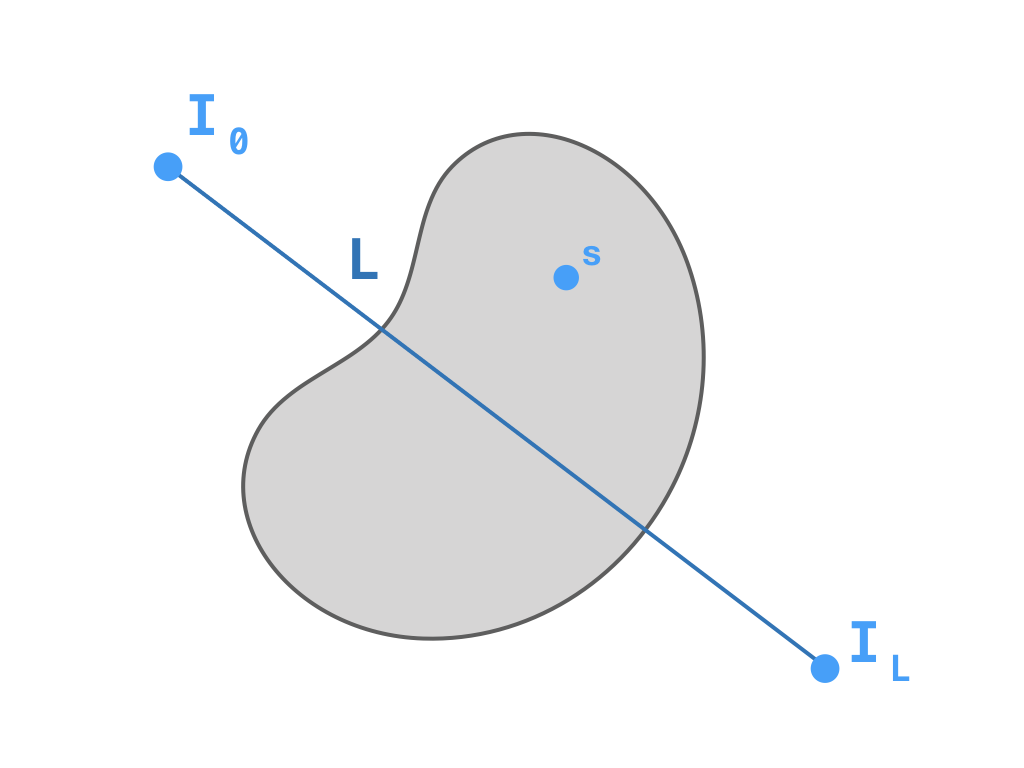
\includegraphics[width=0.7\textwidth]{figures/lambertbeer.png}
    \caption{An illustration of a scanning beam passing through an object}
    \label{fig:lambertbeer}
\end{figure}
The Lambert-Beer law describes the energy attenuation of a beam as it passes through an object. It does this using a function $x(s)$, which given a point $s$ within the object will return the attenuation coefficient at that point. This number is always positive and the larger it is the more energy is consumed as the beam passes through that point. This means that if $x(s)$ for any $s$ is known, then $x(s)$ can be used to create a visual reconstruction of the object. The relationship between the energy of the beam at entry and exit is according to Lambert-Beer given by:
$$
    I_{L} = I_{0} \cdot \text{e}^{-\int_{L}~x(s)~\text{d}s} 
$$
From this we can derive a formula for the projection of the line $L$. First we divide with $I_L$ and then we take the natural logarithm on each side. We arrive at:
\begin{align*}
    P_L = \text{log}~\left(\frac{I_{0}}{I_{L}}\right) = \int_{L}~x(s)~\text{d}s
\end{align*}
Where $P_L$ denotes the projection of line $L$. Since $I_0$ and $I_L$ are known from the scanning process, the integral can be estimated using a sum to make it discrete. Estimating this integral in matrix-vector representation is referred to as reconstruction in the rest of this report.

\subsection{Algebraic Reconstruction Techniques}
The algebraic reconstruction technique (ART) is a class of iterative algorithms for the solution of the discrete reconstruction problem. These reconstruct an image from a series of angular projections, also known as sinograms, and are discrete approximations of the inverse Radon transform, while the sinogram is the Radon transform of the image\cite{PRESS}.

ART can be considered an iterative solver of a system of linear equations:
\begin{align}\label{grail}
    \mathbf{A}\mathbf{x}=\mathbf{y}
\end{align}
The values of the pixels used to model the geometry of the scanned object are considered as variables collected in a vector or 2D array $\mathbf{x}$. The image process is described by a matrix $\mathbf{A}$. In $\mathbf{A}$, each entry is a flat array. These arrays are collections of line-lengths within the pixels that a given line passes through. Each row in the matrix $\mathbf{A}$ collects all the arrays for a given scan angle, and each column corresponds to a scan line. In other words, in the 2D matrix $\mathbf{A}$, the entry $(i,~j)$ is the line-length data of $j$'th line  projected from $i$'th angle.\\
\iffalse
\begin{figure}[h]
    \centering
    \caption{Grid representation of an entry in the $\mathbf{A}$ matrix}
    \label{gridObject}
    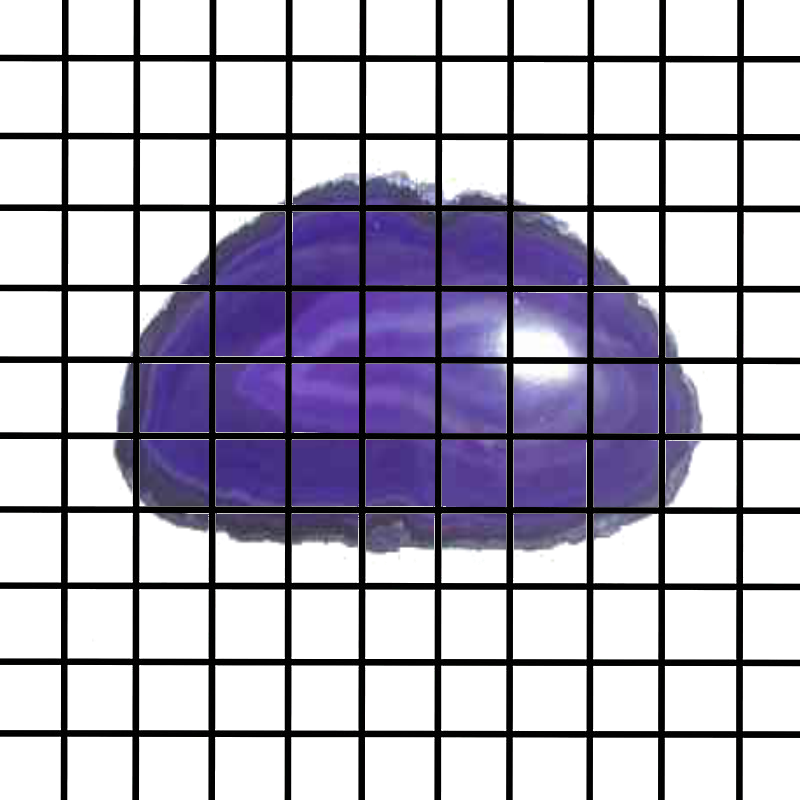
\includegraphics[width=0.4\textwidth]{figures/gridObject.png}
\end{figure}
\fi

The measured energy losses are collected in a vector $\mathbf{y}$, or alternatively a 2D array, with each column corresponding to a projection angle and each line to a projection. Given a $m*n$ matrix $\mathbf{A}$ and a vector $\mathbf{y}$, classical ART computes an approximation of the solution of the linear systems of equations as in the following formula:
\begin{align}
    x^{k+1}=x^k+\lambda_k \frac{y_i-\langle a_i,x^k \rangle}{||a_i||^2}a_i^T
\end{align}
where $\langle \bullet , \bullet \rangle$ denotes the inner product of two vectors, $i=k~\text{mod}~m+1$, and $a_i$ is the $i$'th row of the matrix $\mathbf{A}$, $y_i$ is the $i$'th component of the vector $\mathbf{y}$, and $\lambda_k$ is a relaxation parameter. 
The above formulae give a simple iteration routine, but this function could be expressed in any number of ways, while still remaining an ART function, as long as each iteration of the function results in convergence towards the true image representation of the scanned object\cite[p.~194]{FCT}. 
Thus we instead utilize a least-squares function, allowing us to approximate a solution to even underdetermined systems, where a unique solution could otherwise not be found\cite{BLOCK}.
Expressed as a least squares problem, expression \ref{grail} becomes:
\begin{align}
    \text{argmin}_{\mathbf{x}}~\frac{1}{2} ~ || \mathbf{Ax} - \mathbf{y} ||^{2}
\end{align}
The size of the standard pseudo-inverse solution is prohibitively large however, and thus it is necessary to divide the problem into smaller parts, by dividing $\mathbf{A}$ into vertical blocks $\mathbf{A}_i$ and $\mathbf{y}$ into blocks $\mathbf{y}_i$ as well.
This allows each pair of blocks to be solved separately, after which the solution to the system as a whole can be found by summing said solutions:
\begin{equation}\label{eq:leastsqaures}
    \frac{1}{2} ~ || \mathbf{Ax} - \mathbf{y} ||^{2} = \sum_{i=1}^K \frac{1}{2} ~ || \mathbf{A}_i\mathbf{x} - \mathbf{y}_i ||^{2}
\end{equation}
In parallel beam tomography, it is natural to let each block correspond to a viewing angle. An advantage of ART over other reconstruction methods is that it is relatively easy to incorporate prior knowledge into the reconstruction process, which is on the path to statistical reconstruction techniques. As such, ART can be a stepping stone towards more advanced techniques.


\subsection{A Remark on Alternate Methods}
The main alternative to ART is Filtered Back Projection (FPB). In terms of accuracy in reconstructing the scanned object, ART outperforms FBP, but this accuracy comes at a cost, since ART is significantly slower than FBP. A single update in ART can be thought to have approximately the same time complexity as FBP in its entirety. 
As such, if $k$ updates are needed to reach the desired precision, ART is slower than FBP by a factor of $k$. In practice if $k$ is $20$, ART will be about 20 times slower than FBP, while the gains in accuracy only amount to around 20\%, and these gains decrease as the amount of available data increases \cite[p.~219]{FCT}\cite[p.~210\iffalse table 11.1 \fi]{FCT}. The tradeoff between speed and accuracy underlines why FBP remains in use, even in the presence of a more accurate method, and why our attempt to improve the calculation speed of ART using GPUs is worthwhile. Ideally, we will be able to drastically decrease the runtime of ART, thus mitigating the tradeoff. 

\subsection{Filtered Back Projection}
The simplest algorithm for reconstructing an object is to estimate the density at a point by adding all the ray sums of the lines through that point. This method is referred to as the \textit{back projection method} and is the basis for FBP. While conceptually simple, back projection suffers from a smearing effect, since each point in the image grid receives non-negative contributions from all other points of the original image. This creates a haze that is specifically pronounced around edges. A greater issue is that regular back projection does not converge to the solution of $\mathbf{Ax}=\mathbf{y}$.

Filtered back projection is a practical implementation of the Radon inverse transform designed to overcome the limitations of conventional back-projection; it applies a filter to remove the blurring effect, such as a ramp filter, which is considered the ideal filter for inverse Radon transforms. With ramp filters, points with sufficiently high values are kept, while points below the threshold are attenuated or removed completely, with a linear behavior in between. Thus with this filter, contrasting features are accentuated, while blurring is minimized. An example of back projection with and without filtering is shown on figure \ref{fig:fbp}:

\begin{figure}[H]
    \centering
    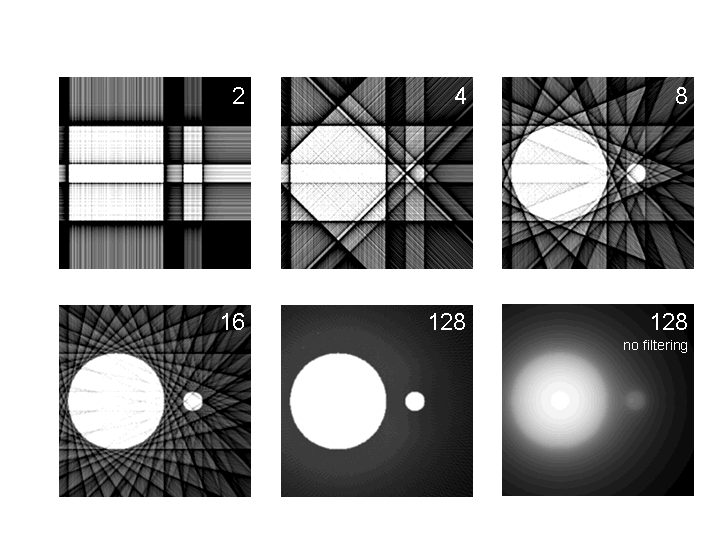
\includegraphics[width=0.7\textwidth]{figures/fbp.png}
    \caption{Filtered Back Projection - With and without filtering\cite{PICTURE}}
    \label{fig:fbp}
\end{figure}
% http://www.impactscan.org/slides/impactcourse/basic_principles_of_ct/img15.html
Iterative reconstruction such as ART typically starts with a regular filtered back projection image, on which it then iterates. So while FBP is seen as an alternative to ART, it also serves as a compliment to it. 